\section{Projekt mentése, megosztása, exportálása}
Az Oracle Data Visualization-ban lehetőségünk van a projektünk mentésére az Oracle felhőben, ki tudjuk exportálni, illetve be tudjuk importálni, valamint meg tudjuk osztani, hogy mások számára is elérhető legyen.

\subsection{Mentés}
Új projekt létrehozása esetán szükséges menteni a projektet, hogy megmaradjon a későbbiek folyamán. Az aktuális projektet a \ref{fig:mentesgomb}. ábrán látható piros téglalappal bekeretezett gomb segítségével tudjuk menteni.

\begin{figure}[!h]
	\centering
	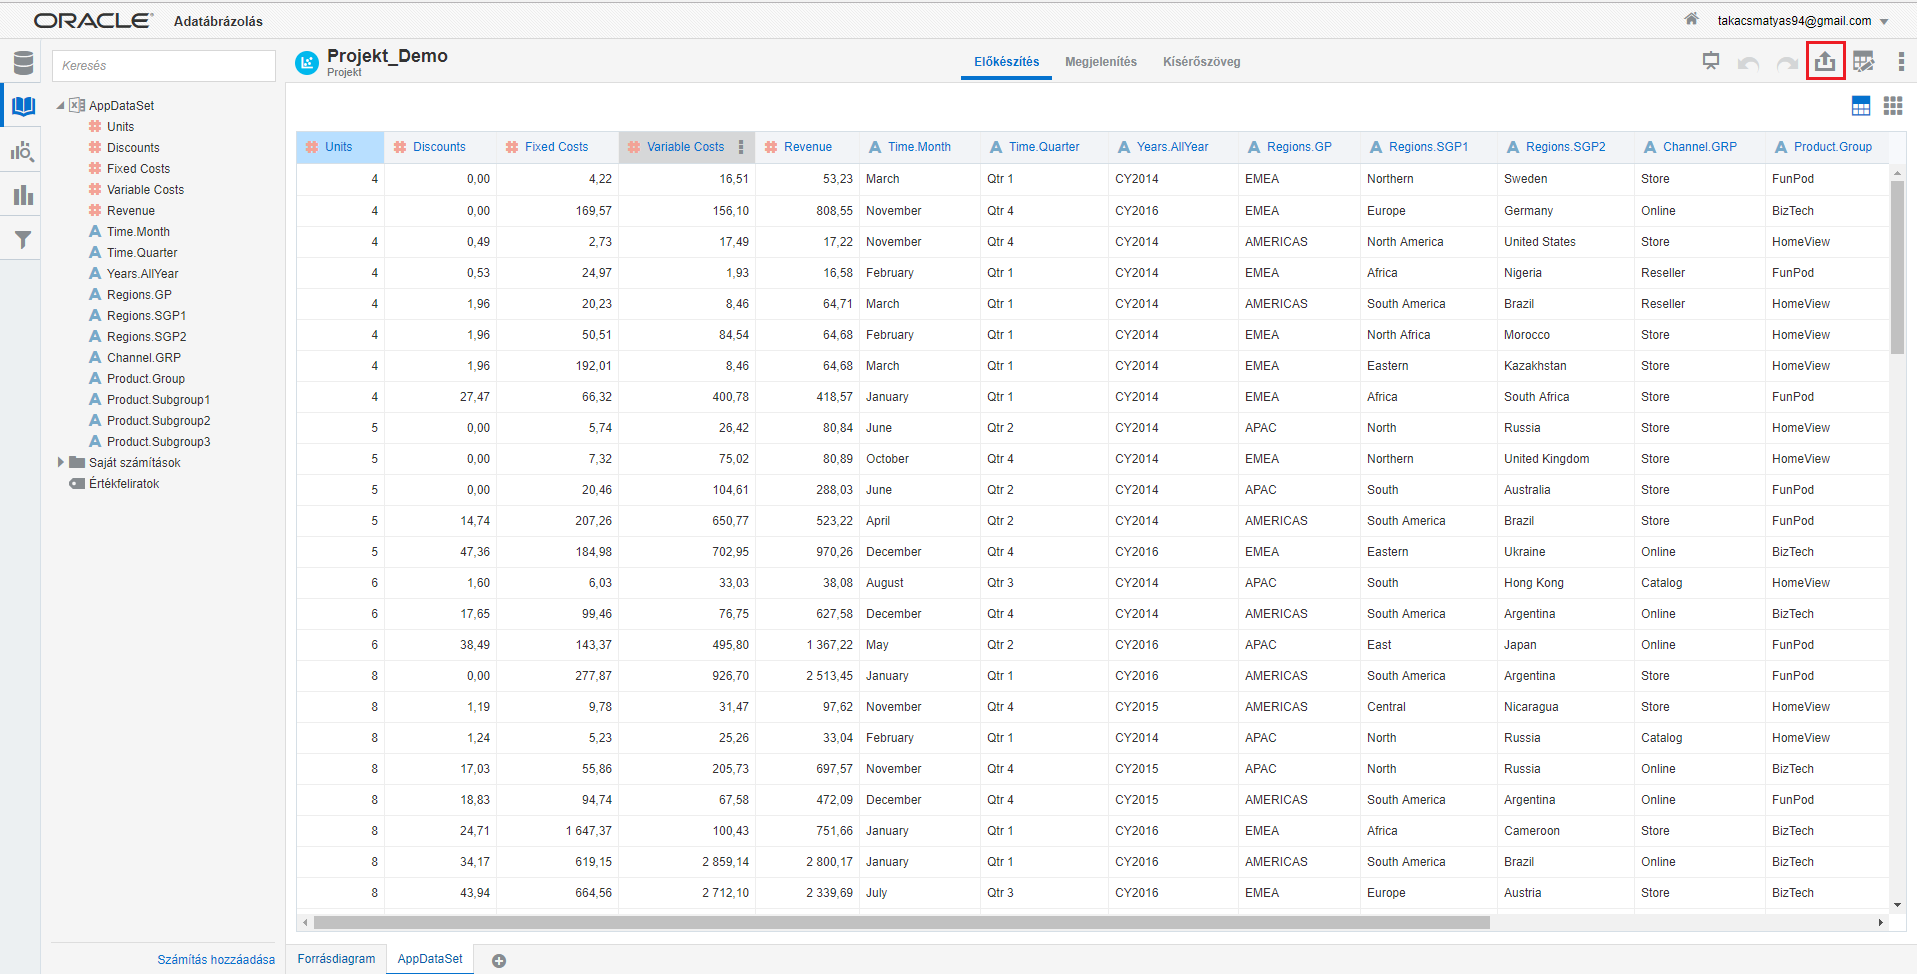
\includegraphics[width=1.0\linewidth]{matyi_imgs/mentesgomb}
	\caption[Projekt mentés gomb]{Projekt mentés gomb}
	\label{fig:mentesgomb}
\end{figure}

Lehetőségünk van a ,,projekt mentése másként'' opcióra is, amely során ki tudjuk választani a felhőben azt a helyet ahova menteni szeretnénk a projektünket illetve a projektünkhöz leírást is tudunk adni(\ref{fig:mentesmaskent}. ábra).

\begin{figure}[!h]
	\centering
	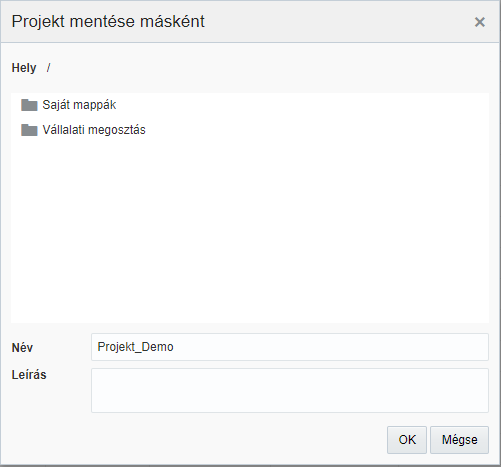
\includegraphics[width=0.7\linewidth]{matyi_imgs/mentesmaskent}
	\caption[Projekt mentése kiválasztott helyre]{Projekt mentése kiválasztott helyre}
	\label{fig:mentesmaskent}
\end{figure}

Mentési helynek meg tudjuk adni a saját mappánkat, vagy a vállalati megosztás mappát is, így a projektünk elérhetővé válik a vállalat résztvevőinek számára is.

\pagebreak

\subsection{Megosztás}
Saját projektet kétféleképpen tudunk megosztani a vállalattal. Az egyik módszer, ha a projektünket lementjük másként a vállalati megosztás mappába. Ezt gyakorlatilag a mentés másként gombot megnyomva tudjuk ezt megtenni.

A másik módszer során lényegében áthelyezzük a projektünket a vállalati megosztás mappába. Ezt a következőképp tudjuk megtenni. A Data Visualization Cloud Service kezdőlapján láthatóak a projektjeink(\ref{fig:kezdolap}.ábra)
\begin{figure}[!h]
	\centering
	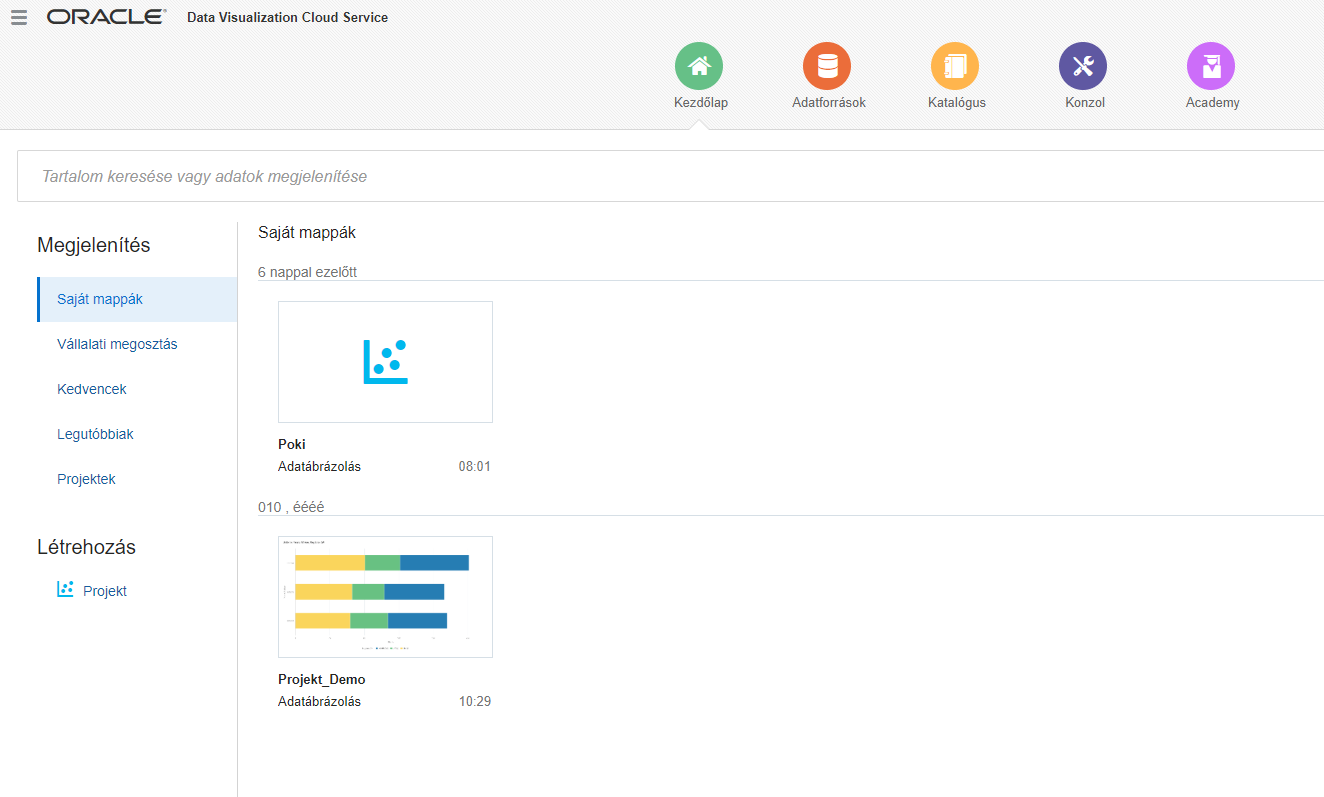
\includegraphics[width=0.7\linewidth]{matyi_imgs/kezdolap}
	\caption[A kezdőlapon látható projektek]{A kezdőlapon látható projektek}
	\label{fig:kezdolap}
\end{figure}
. Itt a megosztani kívánt projektre ráhúzva az egeret rákattintunk az ,,áthelyezés ide...'' gombra(\ref{fig:athelyezes}.ábra). 
ez után kiválasztjuk a vállalati megosztás mappát és rákattintunk az áthelyezés gombra. Ha meg szeretnénk tartani a saját mappánkban a projektet akkor az áthelyezés előtt egy másolatot kell létrehoznunk a projektünkből. 
 
\begin{figure}[!h]
	\centering
	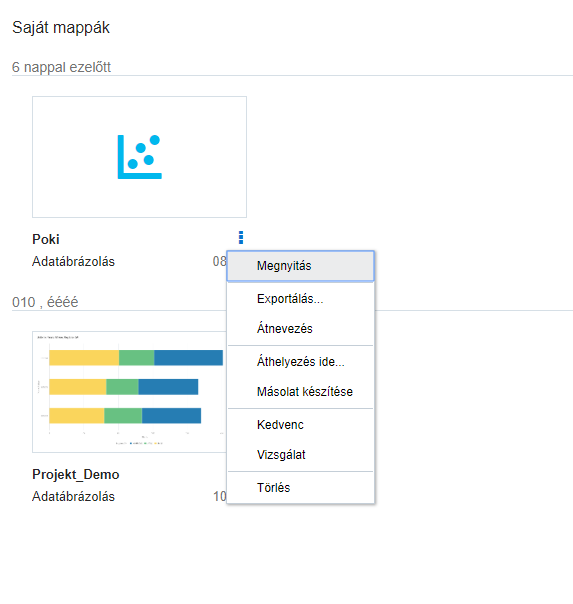
\includegraphics[width=0.6\linewidth]{matyi_imgs/athelyezes}
	\caption[Projekt műveletek]{Projekt műveletek}
	\label{fig:athelyezes}
\end{figure}

\subsection{Exportálás}
Lehetőségünk van projektjeink exportálására is, ez által hordozhatóvá tudjuk tenni az itt elkészített projektjeinket. Az exportálást ugyanabból a menüből el tudjuk érni, mint amiből a projektet tudjuk áthelyezni. Az exportálás gombra rákattintva a \ref{fig:exportalas}.ábrán látható ablak fogad minket.

\begin{figure}[!h]
	\centering
	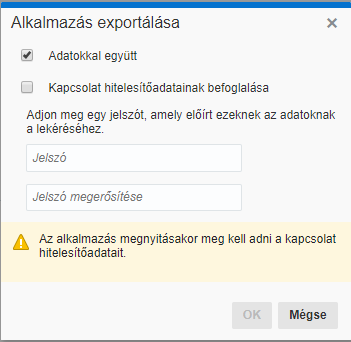
\includegraphics[width=0.7\linewidth]{matyi_imgs/exportalas}
	\caption[Projekt exportálása]{Projekt exportálása}
	\label{fig:exportalas}
\end{figure}

Itt ki tudjuk választani, hogy az adatokkal együtt, vagy a nélkül szeretnénk exportálnia  projektet. Be tudjuk állítani azt is, hogy az alkalmazás megnyitásakor meg kelljen adnunk a hitelesítő adatokat vagy sem. Ahhoz hogy ki tudjuk exportálni a projektünket kötelezően meg kell adnunk egy jelszút, azonban a jelszó tartalmi követelményére nincs megszorítás. A lementett projektünk .dva formátumban kerül tárolásra.

\pagebreak

\subsection{Importálás}
Az importálás során a lementett projekteket tudjuk betölteni. Az importálást a kezdőlap jobb felső sarkában lévő menüből tudjuk elérni(\ref{fig:importalas}).

\begin{figure}[!h]
	\centering
	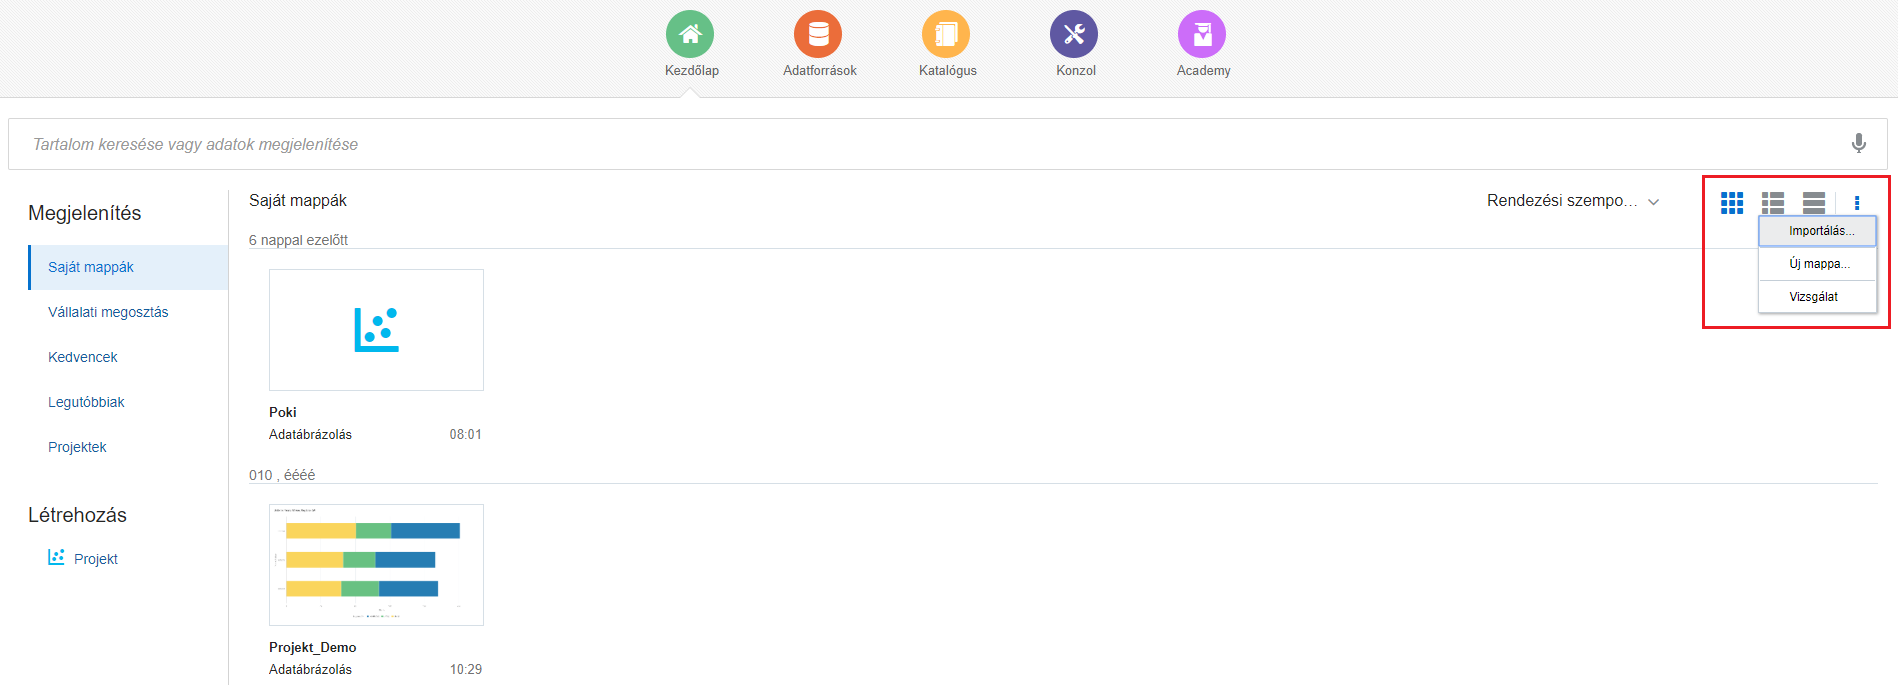
\includegraphics[width=0.7\linewidth]{matyi_imgs/importalas}
	\caption[Importálás elérése]{Importálás elérése}
	\label{fig:importalas}
\end{figure}

Az importálás gombra rákattintva a \ref{fig:importalas2}. ábrán láthetó ablak fogad minket. 

\begin{figure}[h!]
	\centering
	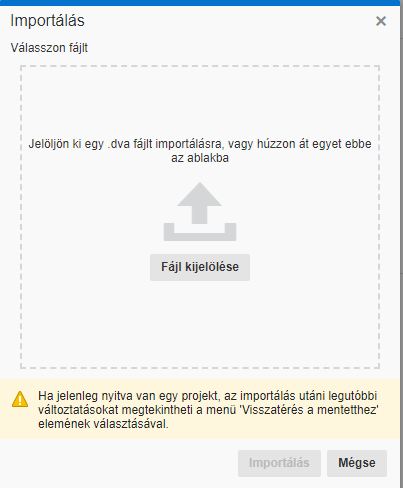
\includegraphics[width=0.5\linewidth]{matyi_imgs/importalas2}
	\caption[Projekt importálása]{Projekt importálása}
	\label{fig:importalas2}
\end{figure}

Itt a kívánt fájlt be tudjuk húzni az ablakba, de be is tudjuk tallózni azt. Ezt követően meg kell adnunk az exportálás során beállított jelszót, majd az importálás gombbal be tudjuk importálni a kívánt projektet.